\chapter*{Valparaiso\markboth{Valparaiso}{}}
\section*{14 mars 2015}
Après Santiago, nouvelle étape \og ville \fg\ avec Valparaiso et juste à côté Viña del Mar.

 \subsection*{Valparaiso}
 La ville est dans la brume tous les matins.
\begin{center} 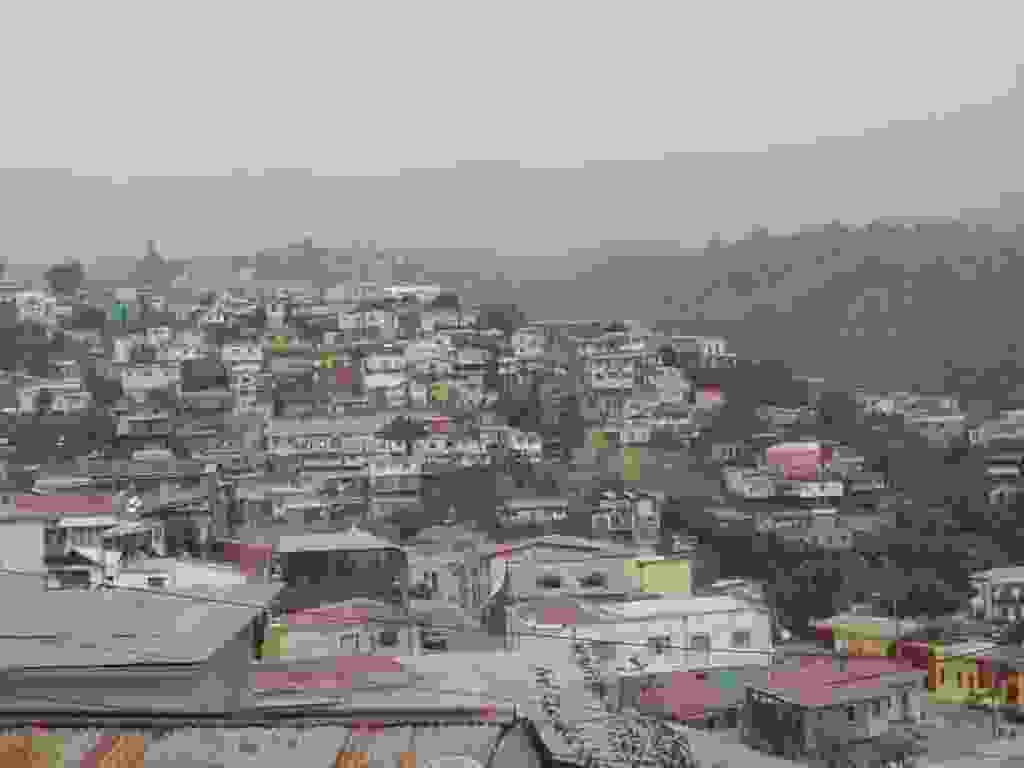
\includegraphics[width=\mywidth]{../wp-content/uploads/2015/03/P3092690-1024x768.jpg} \end{center}
\begin{center} 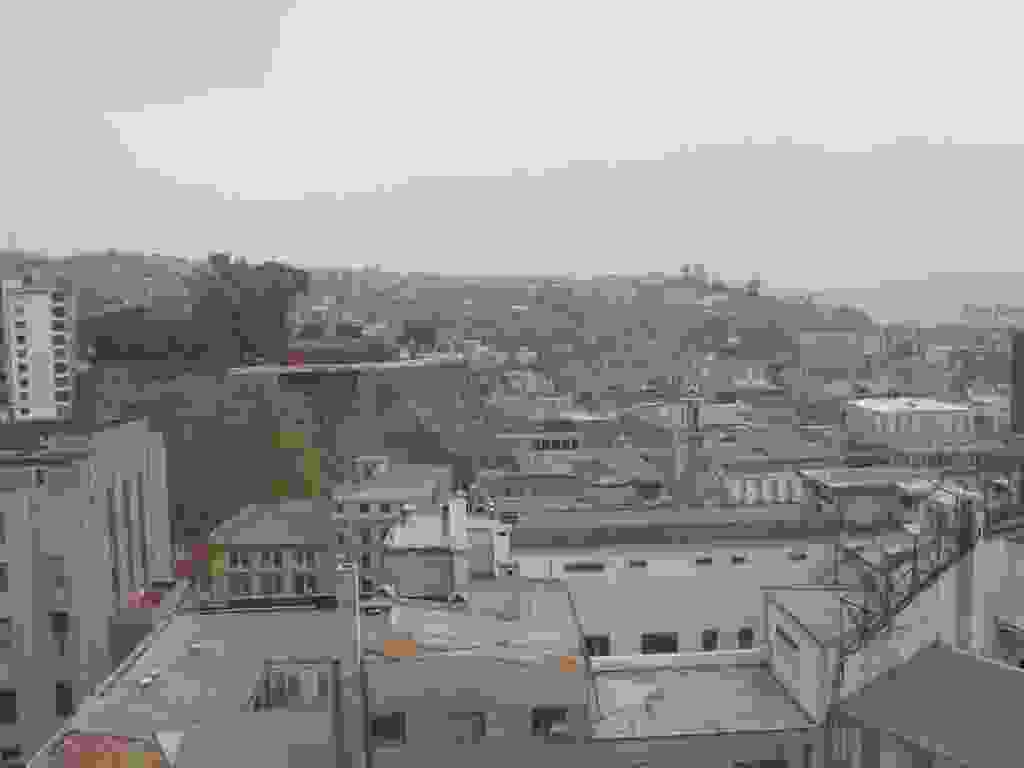
\includegraphics[width=\mywidth]{../wp-content/uploads/2015/03/P30926731-1024x768.jpg} \end{center}

Puis l'après-midi ça se dégage.
\begin{center} 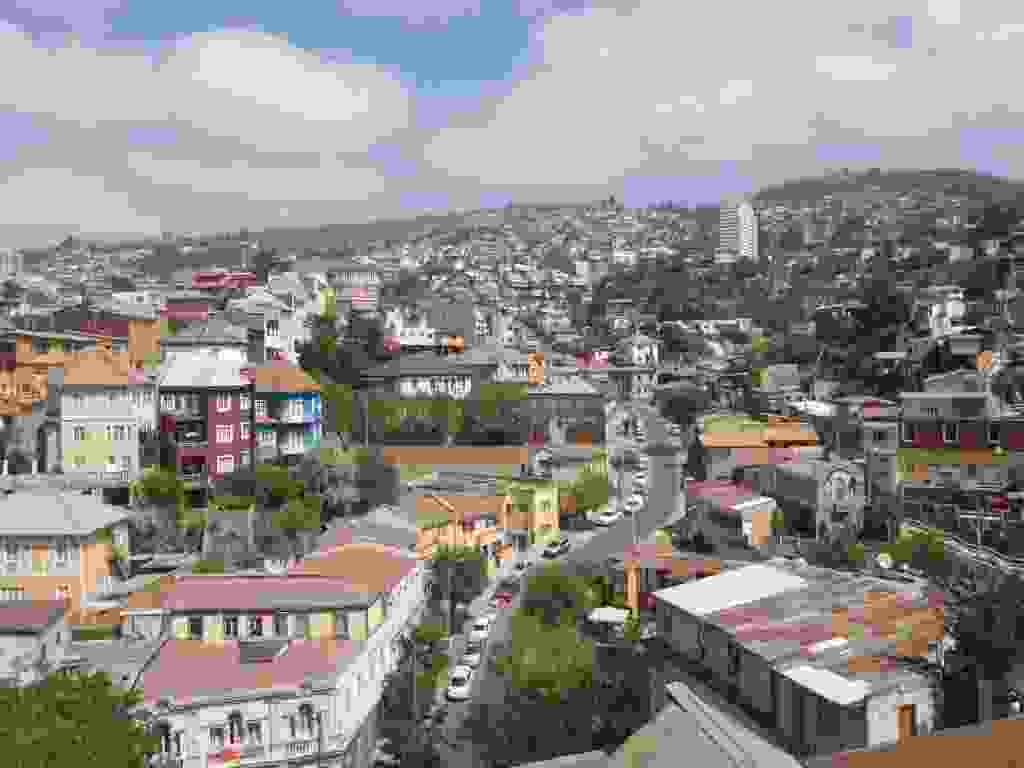
\includegraphics[width=\mywidth]{../wp-content/uploads/2015/03/P3112753-1024x768.jpg} \end{center}
\begin{center} 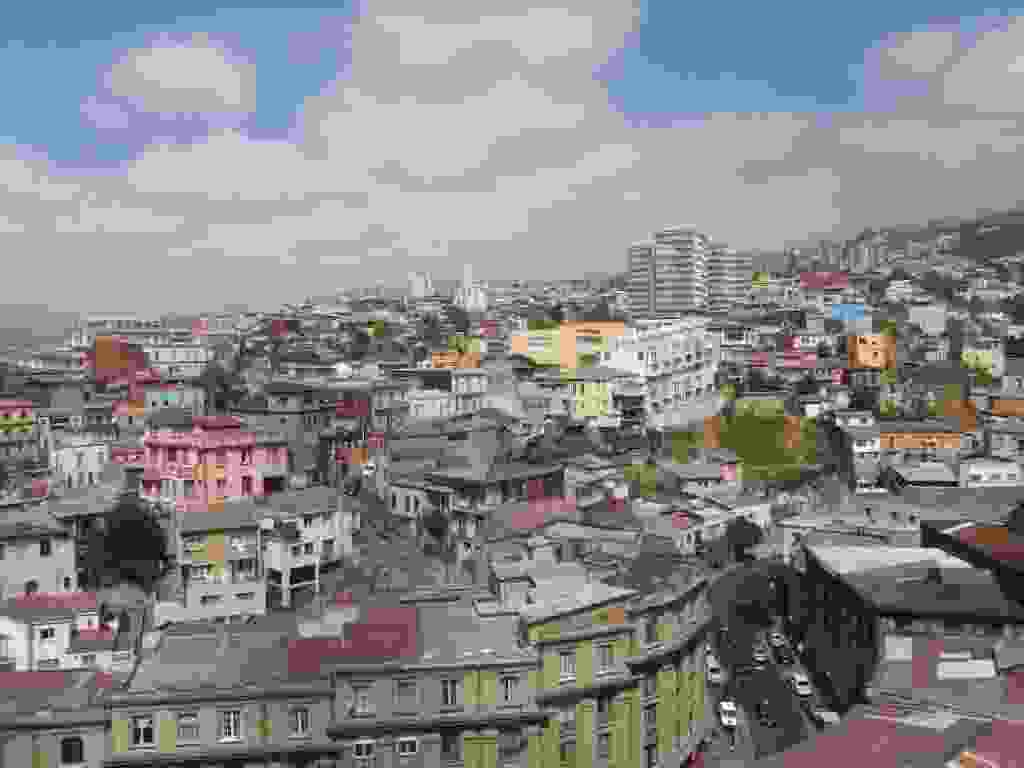
\includegraphics[width=\mywidth]{../wp-content/uploads/2015/03/P3112755-1024x768.jpg} \end{center}
\begin{center} 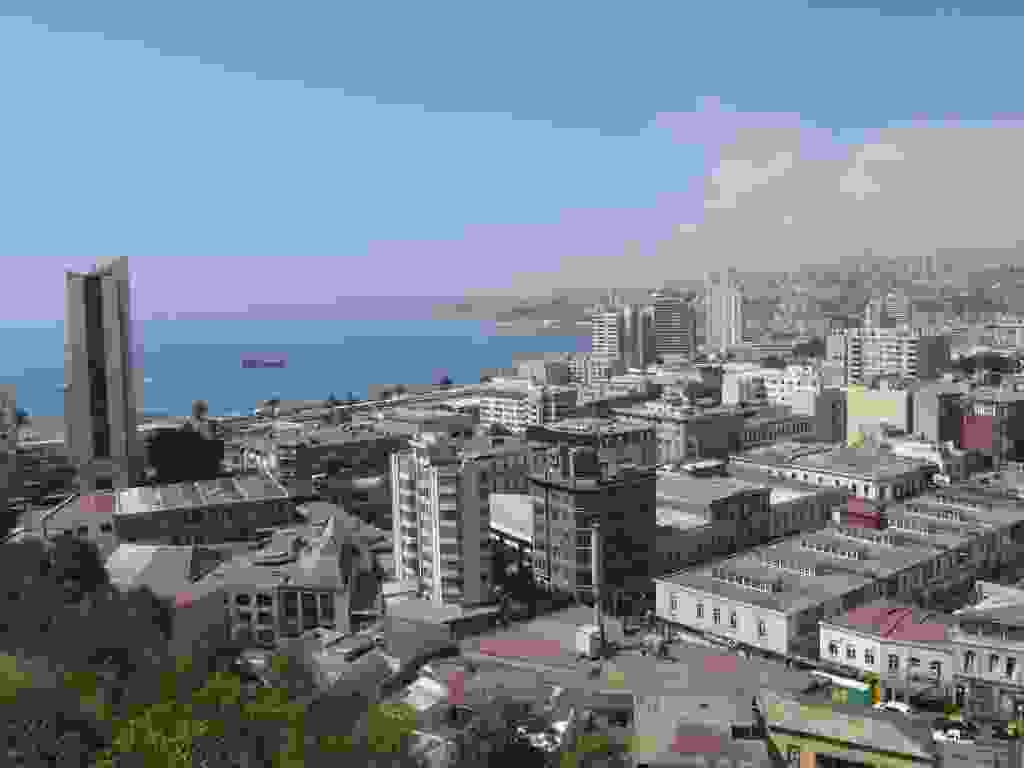
\includegraphics[width=\mywidth]{../wp-content/uploads/2015/03/P3112756-1024x768.jpg} \end{center}
\begin{center} 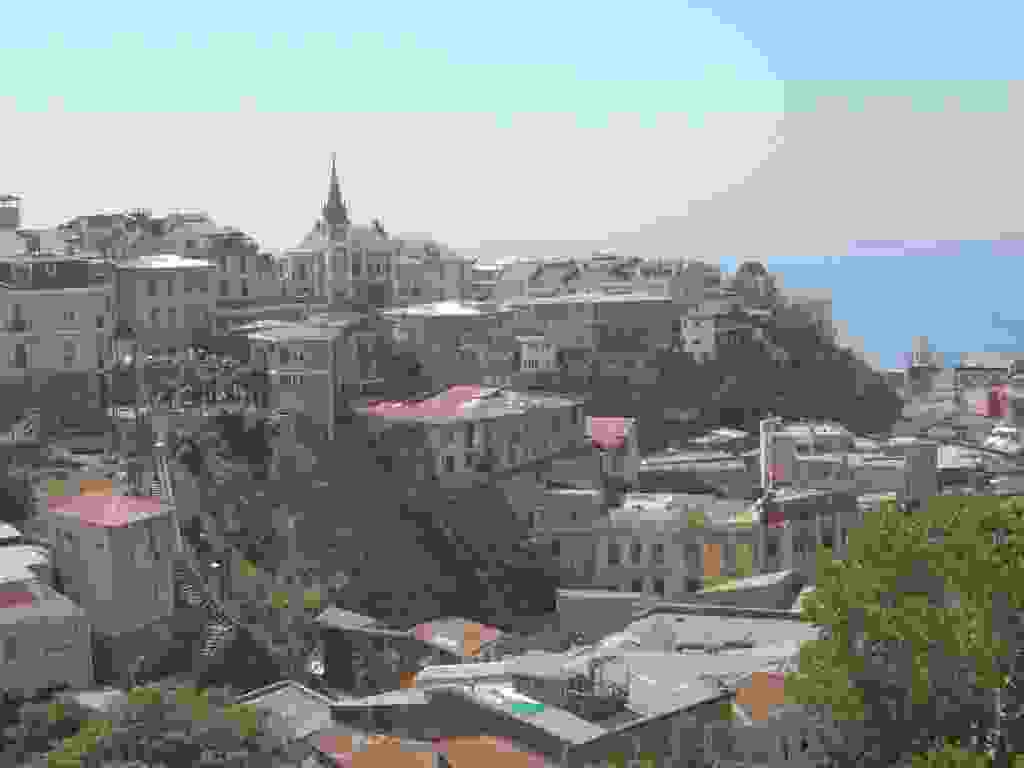
\includegraphics[width=\mywidth]{../wp-content/uploads/2015/03/P3112748-1024x768.jpg} \end{center}
\begin{center} 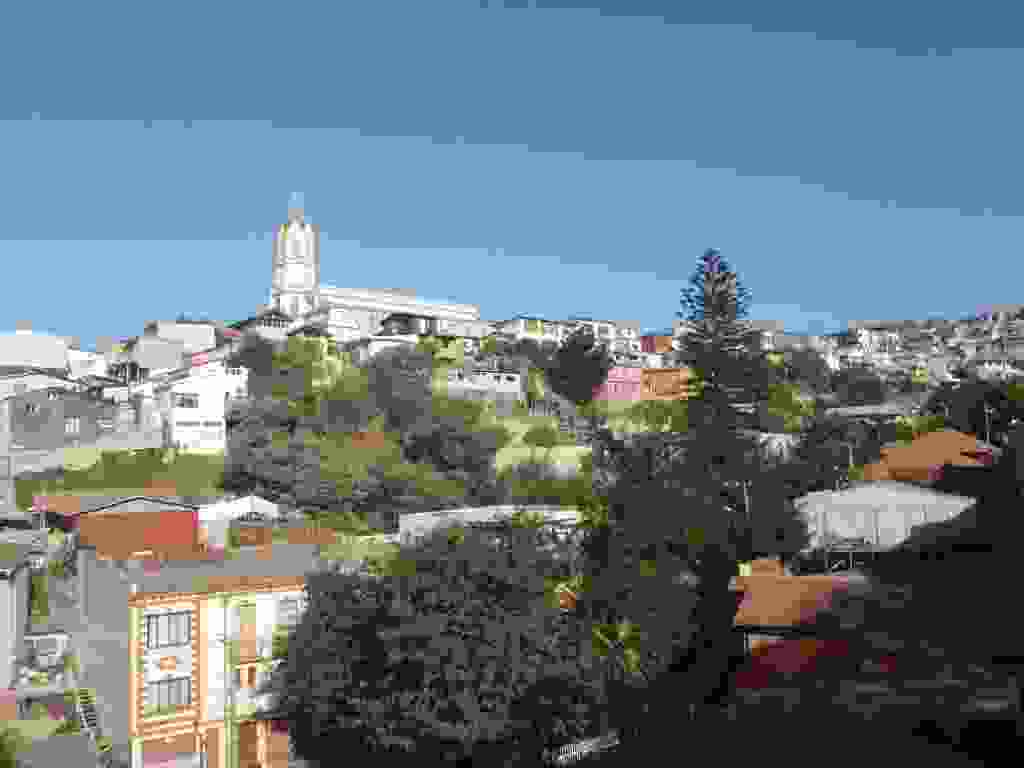
\includegraphics[width=\mywidth]{../wp-content/uploads/2015/03/P3092710-1024x768.jpg} \end{center}
\begin{center} 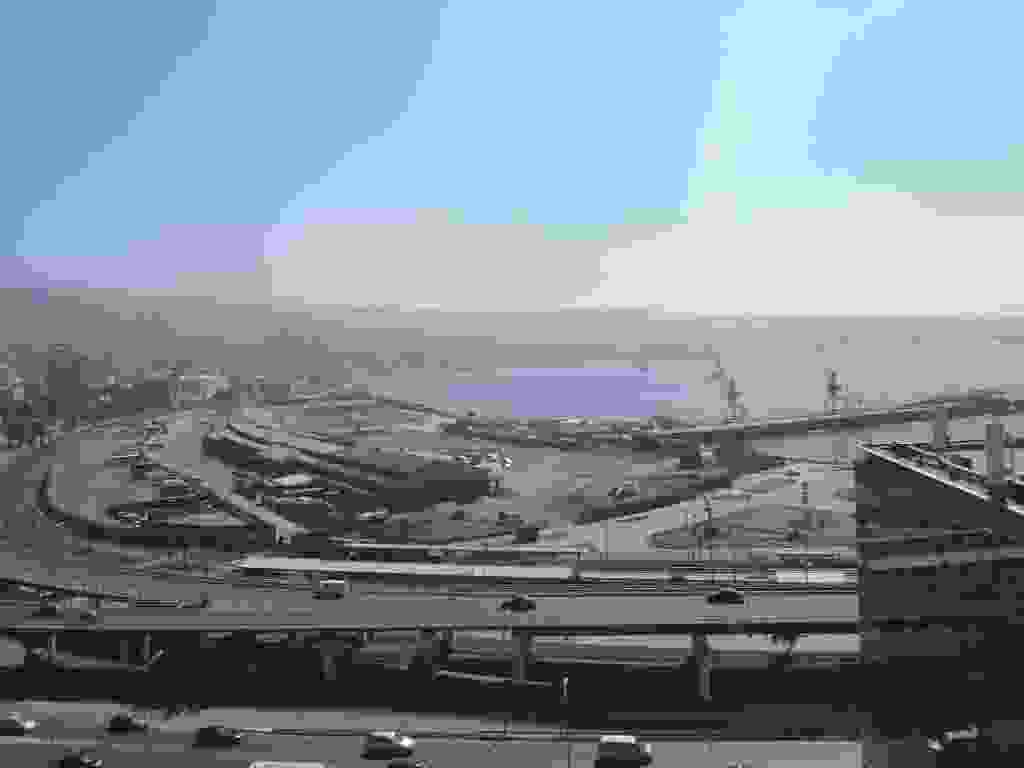
\includegraphics[width=\mywidth]{../wp-content/uploads/2015/03/P3092695-1024x768.jpg} \end{center}

La ville est très colorée avec de nombreuses fresques sur les murs. Il y a aussi des coins assez sales.
\begin{center} 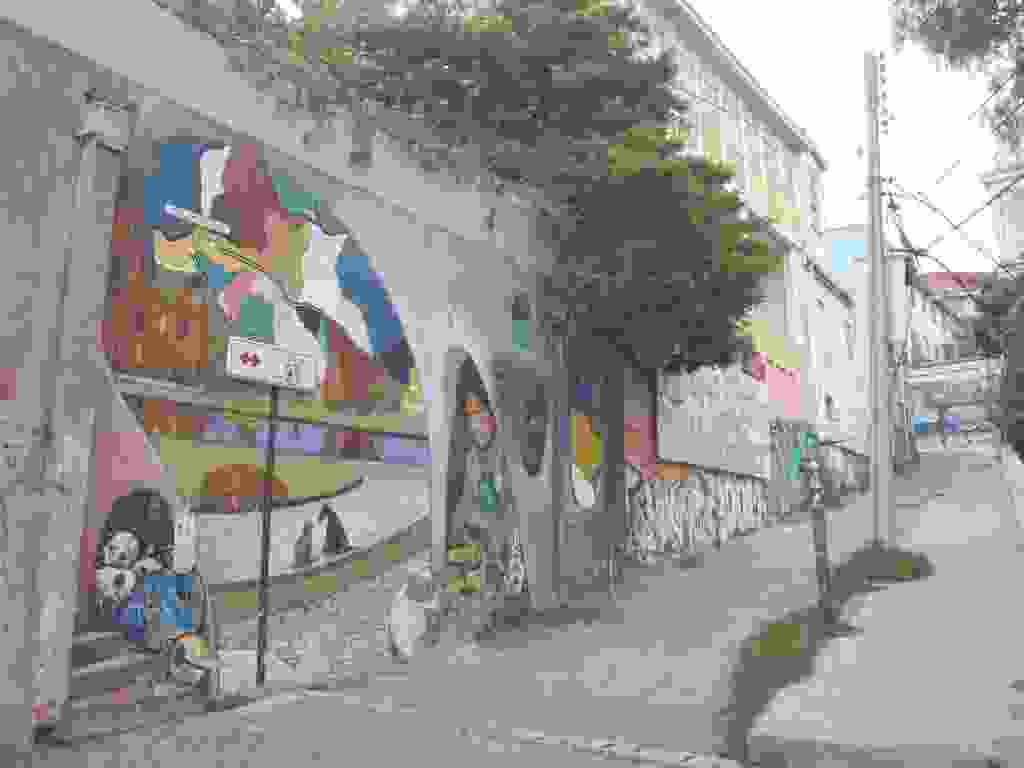
\includegraphics[width=\mywidth]{../wp-content/uploads/2015/03/P3092675-1024x768.jpg} \end{center}
\begin{center} 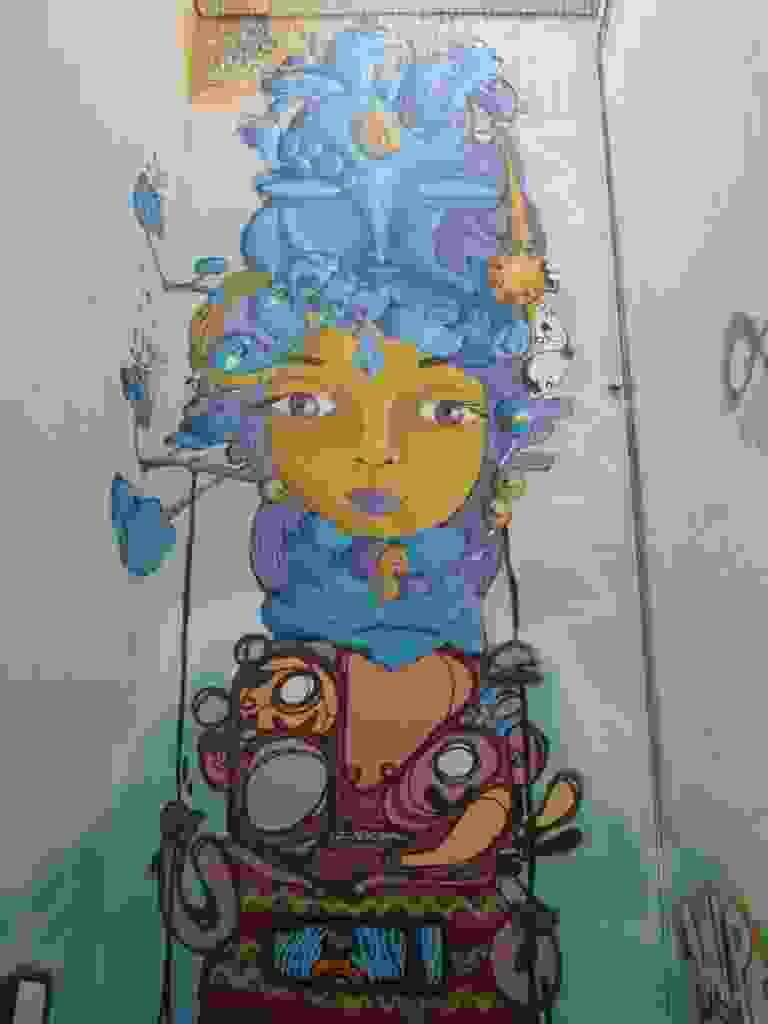
\includegraphics[height=\mywidth]{../wp-content/uploads/2015/03/P3092677-768x1024.jpg} \end{center}
\begin{center} 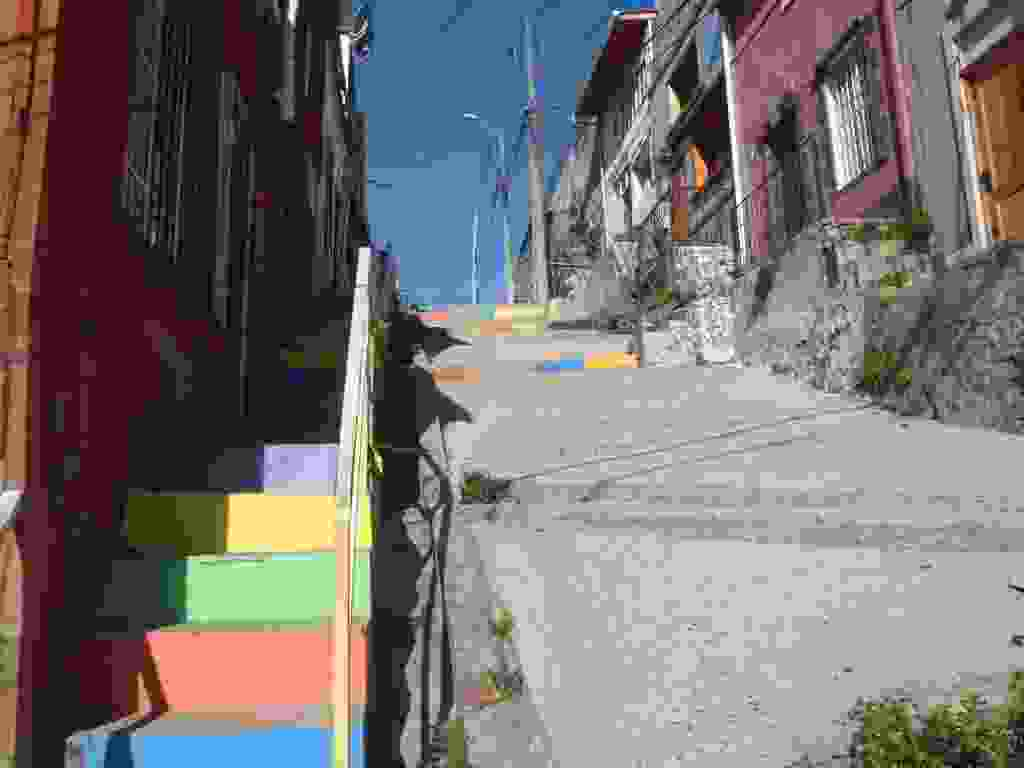
\includegraphics[width=\mywidth]{../wp-content/uploads/2015/03/P3092708-1024x768.jpg} \end{center}
\begin{center} 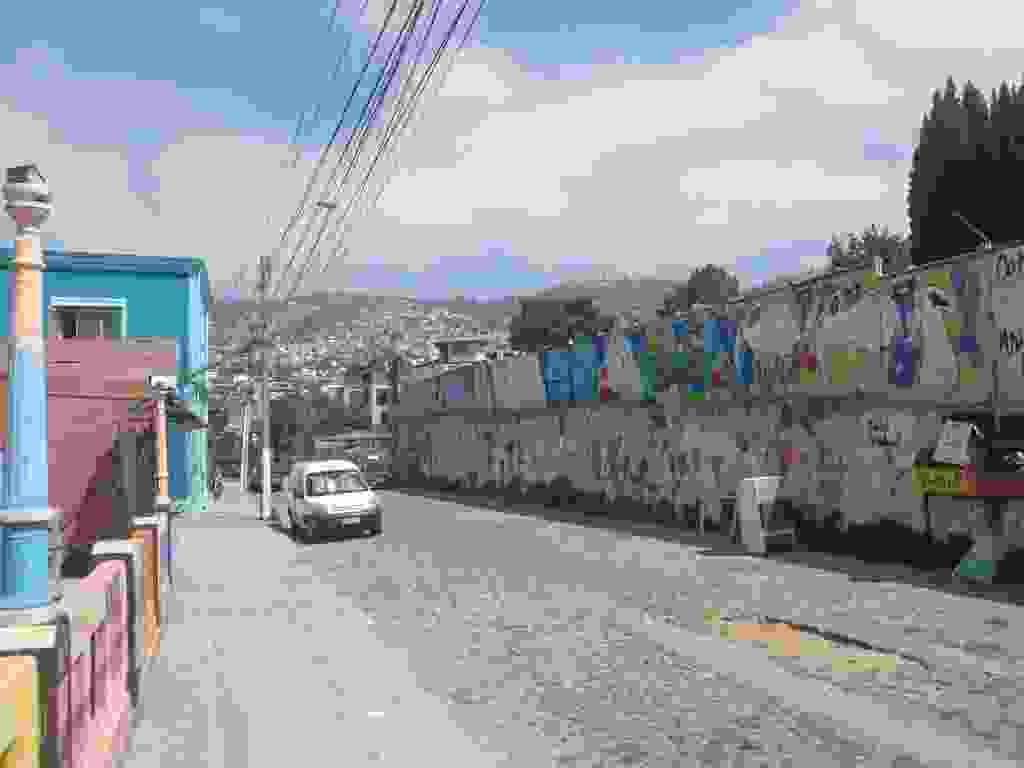
\includegraphics[width=\mywidth]{../wp-content/uploads/2015/03/P3112757-1024x768.jpg} \end{center}
\begin{center} 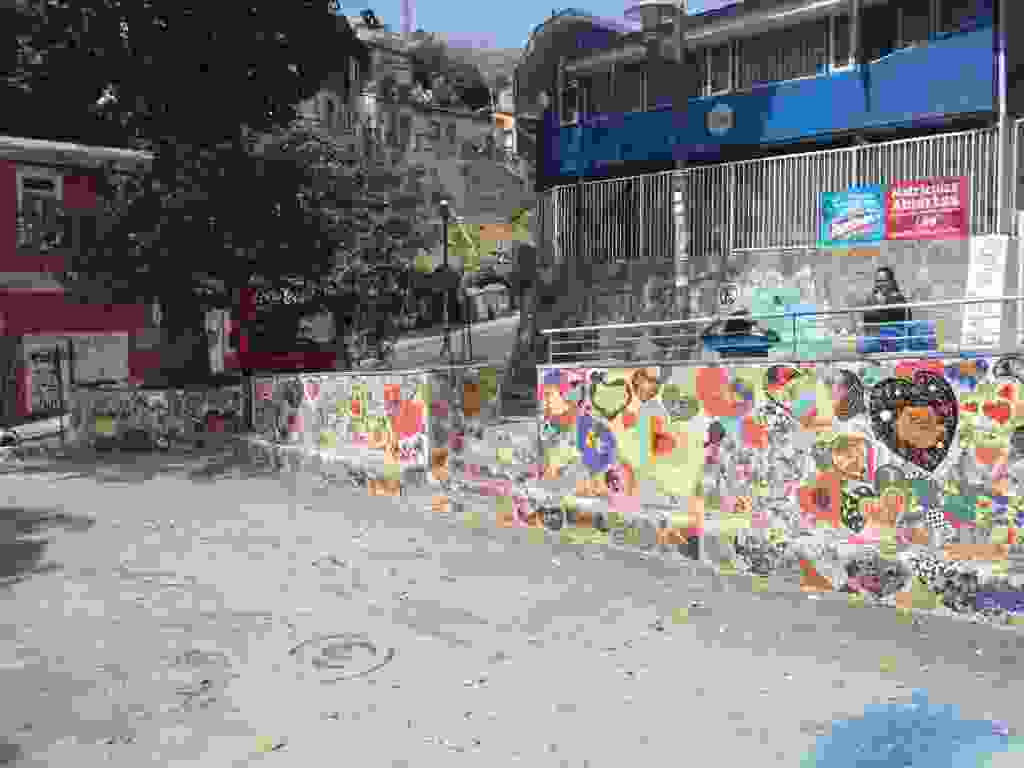
\includegraphics[width=\mywidth]{../wp-content/uploads/2015/03/P3112744-1024x768.jpg} \end{center}
\begin{center} 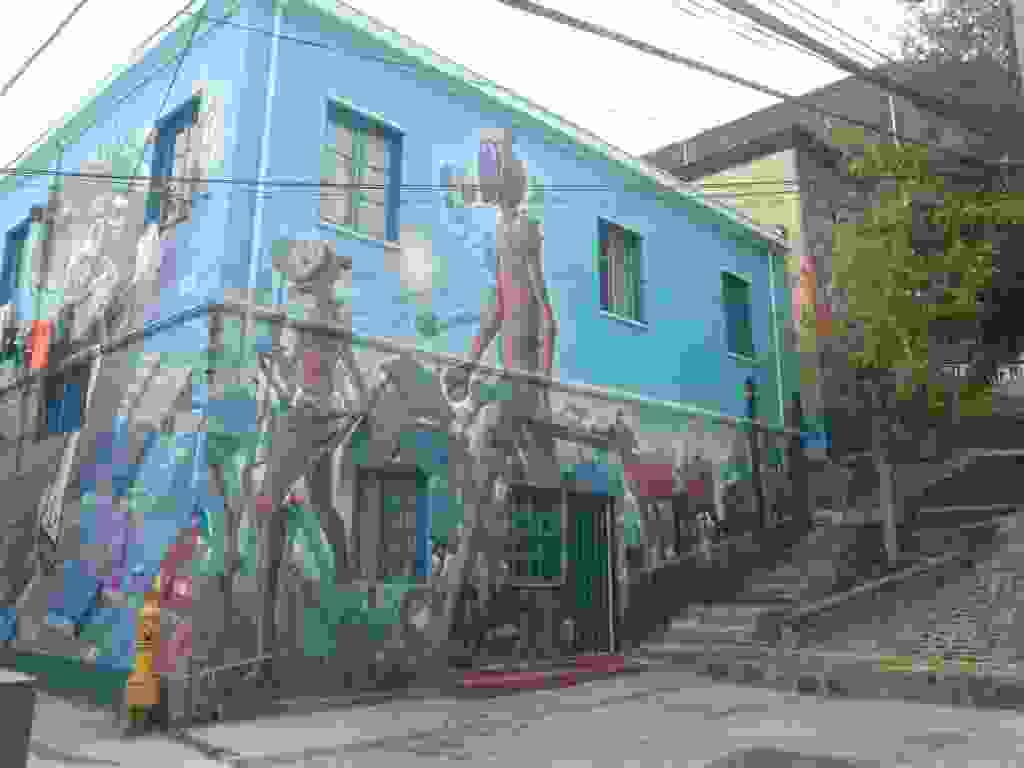
\includegraphics[width=\mywidth]{../wp-content/uploads/2015/03/P3092686-1024x768.jpg} \end{center}

 La Plaza Sotomayor en plein centre.
\begin{center} 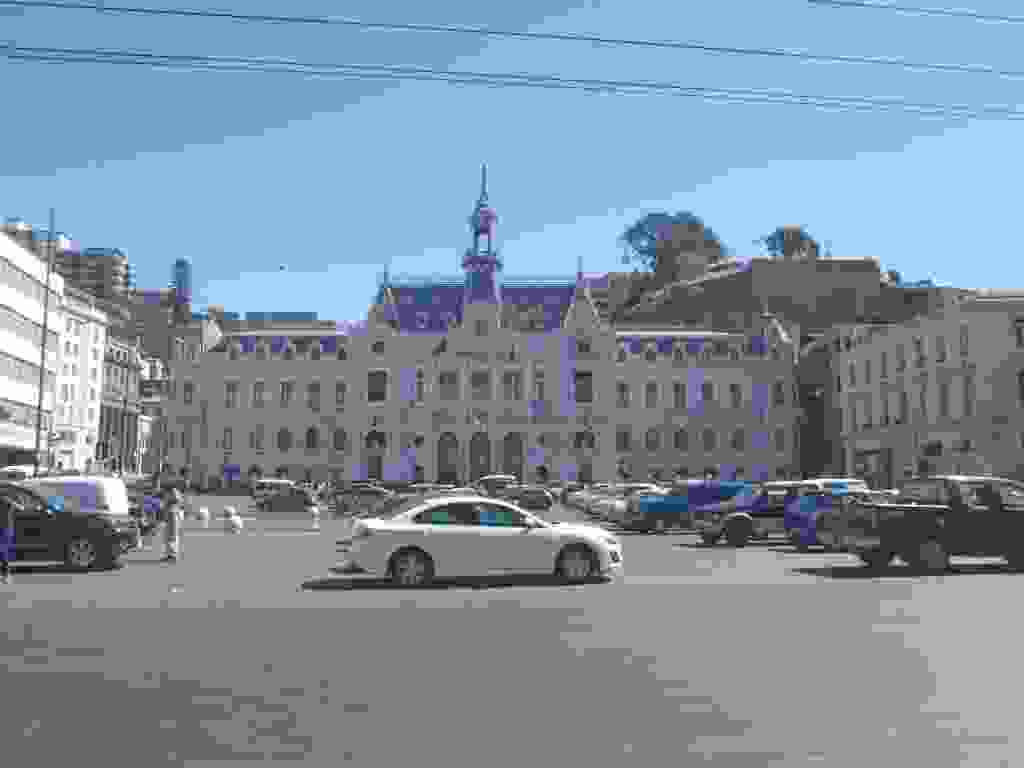
\includegraphics[width=\mywidth]{../wp-content/uploads/2015/03/P3082665-1024x768.jpg} \end{center}
\begin{center} 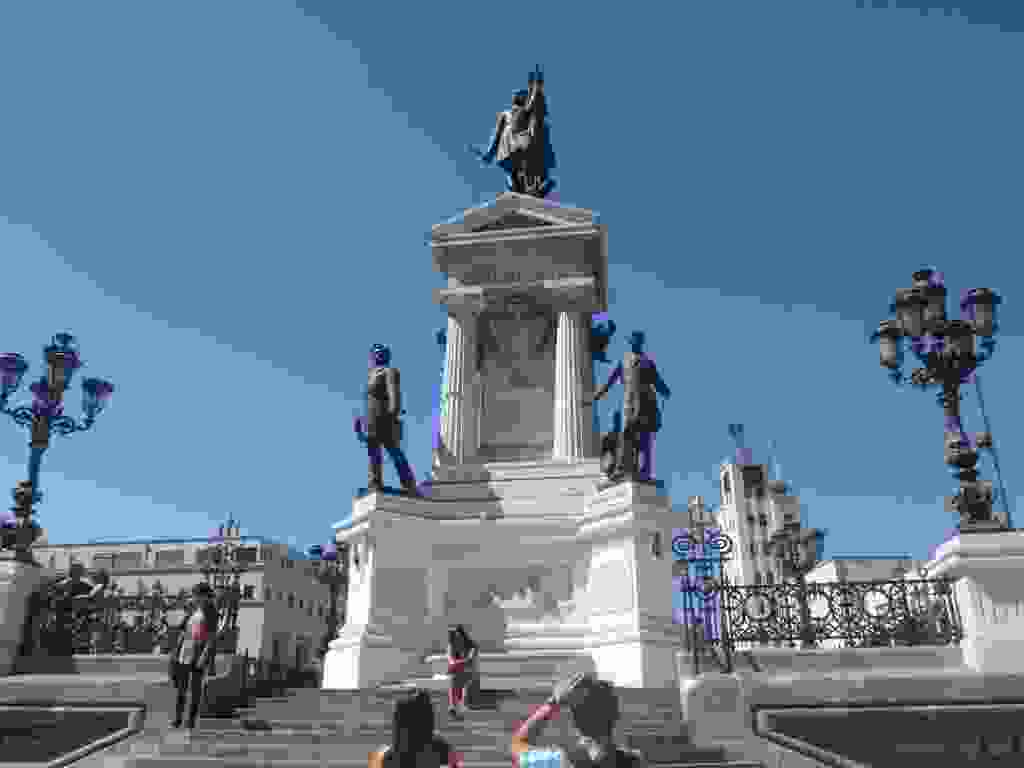
\includegraphics[width=\mywidth]{../wp-content/uploads/2015/03/P3082666-1024x768.jpg} \end{center}

 De multiples petits funiculaires permettent d'accéder aux hauteurs de la ville.
\begin{center} 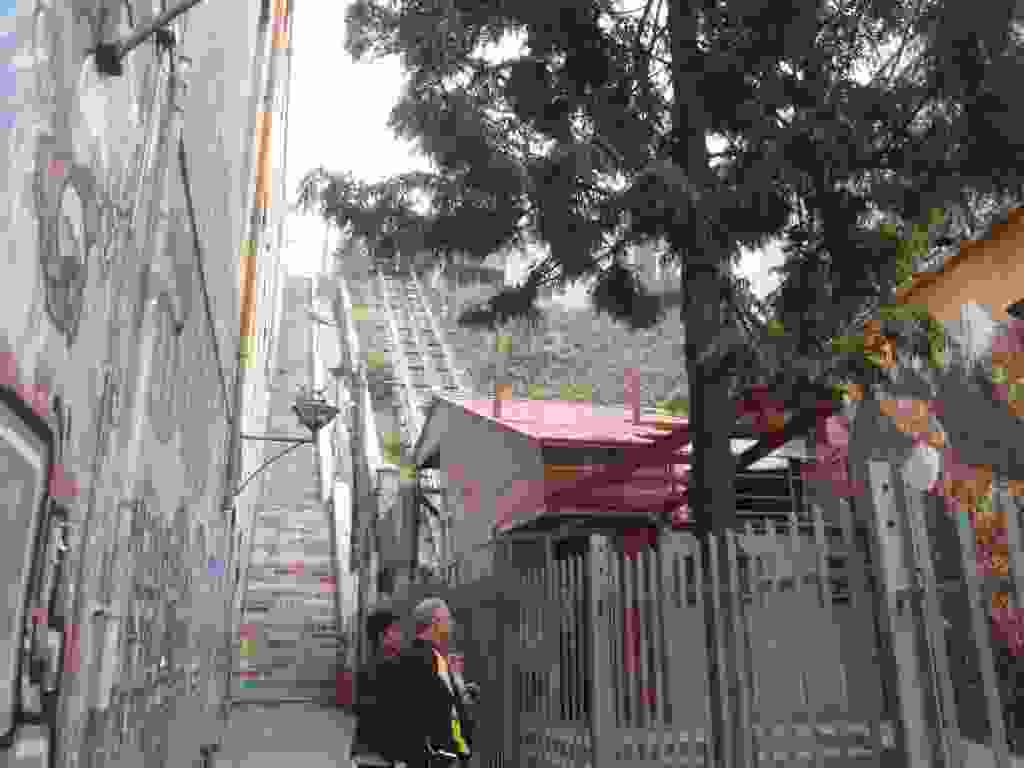
\includegraphics[width=\mywidth]{../wp-content/uploads/2015/03/P3092679-1024x768.jpg} \end{center}
\vspace{-\topsep}

\pagebreak
\begin{center} 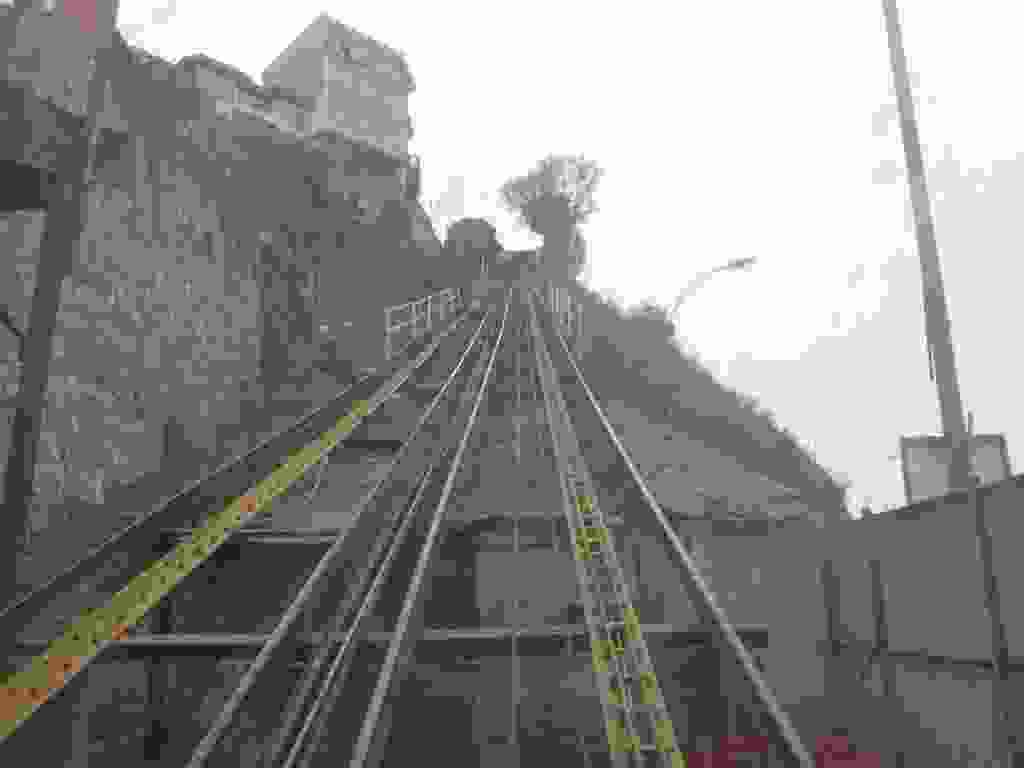
\includegraphics[width=\mywidth]{../wp-content/uploads/2015/03/P3092682-1024x768.jpg} \end{center}
~\\

\begin{center} 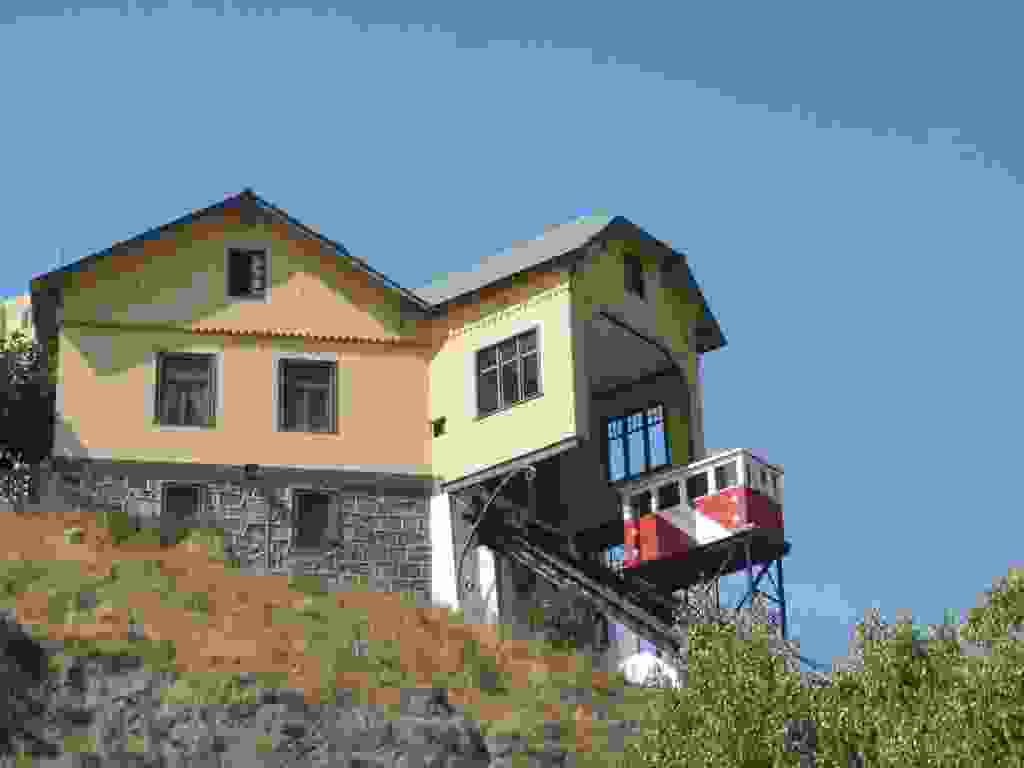
\includegraphics[width=\mywidth]{../wp-content/uploads/2015/03/P3092693-1024x768.jpg} \end{center}
\vspace{-\topsep}
\vspace{-2.75mm}

\pagebreak
Le marché aux fruits.
\begin{center} 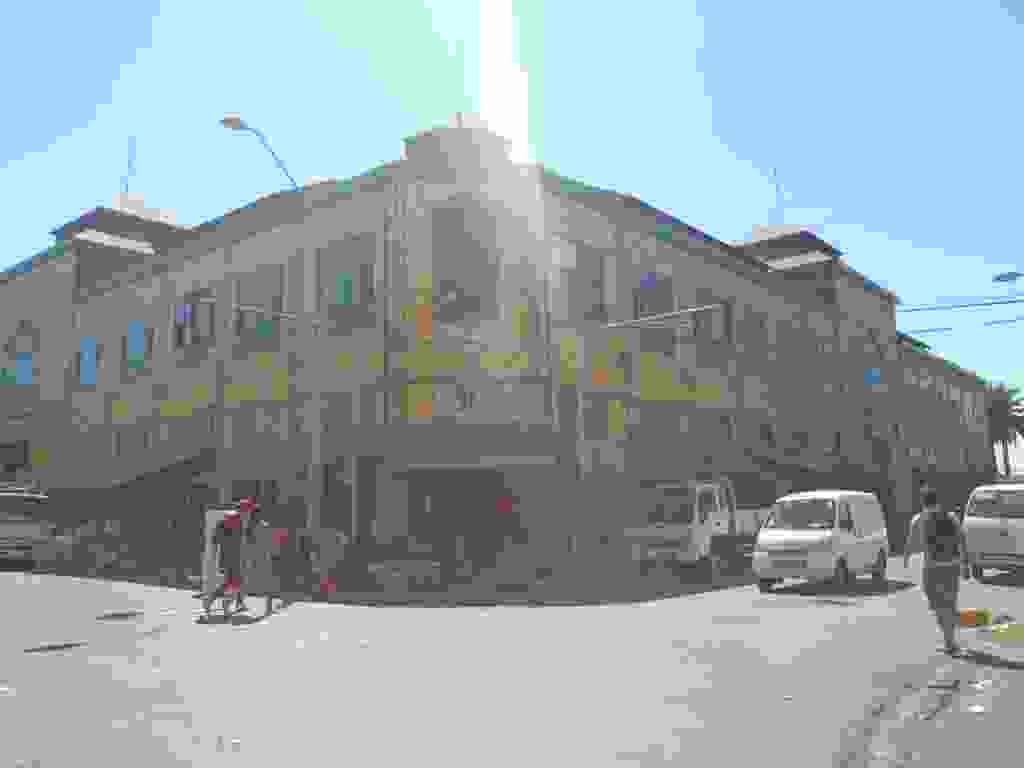
\includegraphics[width=\mywidth]{../wp-content/uploads/2015/03/P3082664-1024x768.jpg} \end{center}

Ils font du bon boulot !
\begin{center} 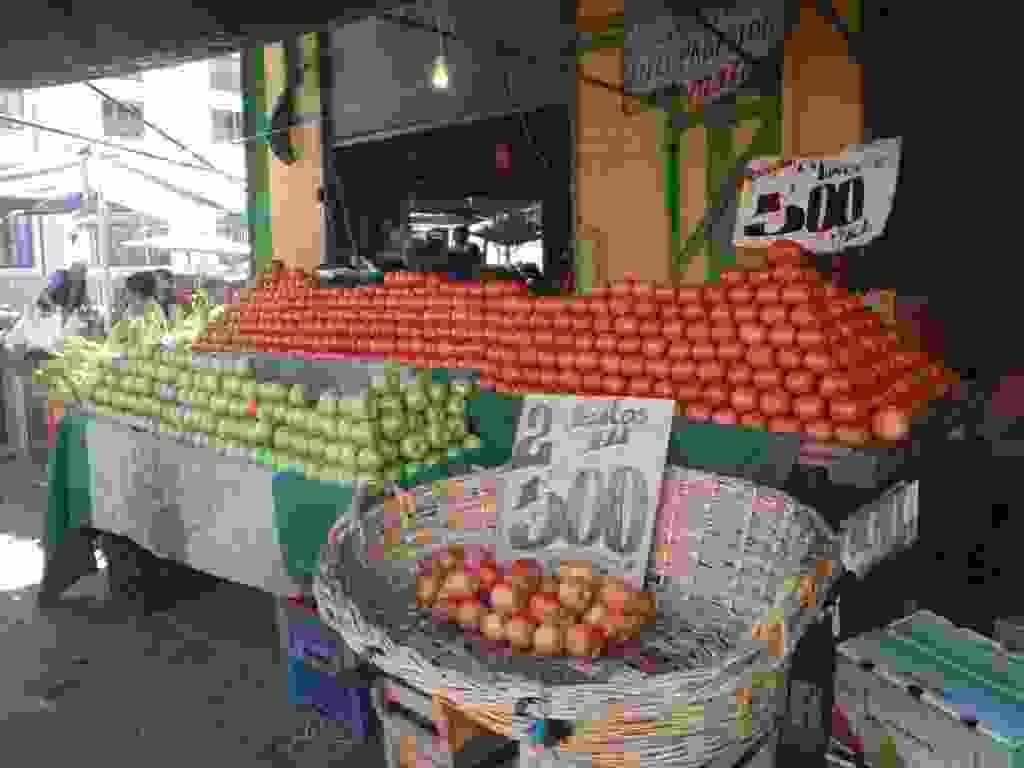
\includegraphics[width=\mywidth]{../wp-content/uploads/2015/03/P3092698-1024x768.jpg} \end{center}
\vspace{-\topsep}

\pagebreak
 L'hostel où j'ai logé à Valparaiso, tenu par un français et aussi avec beaucoup de clients français.
\begin{center} 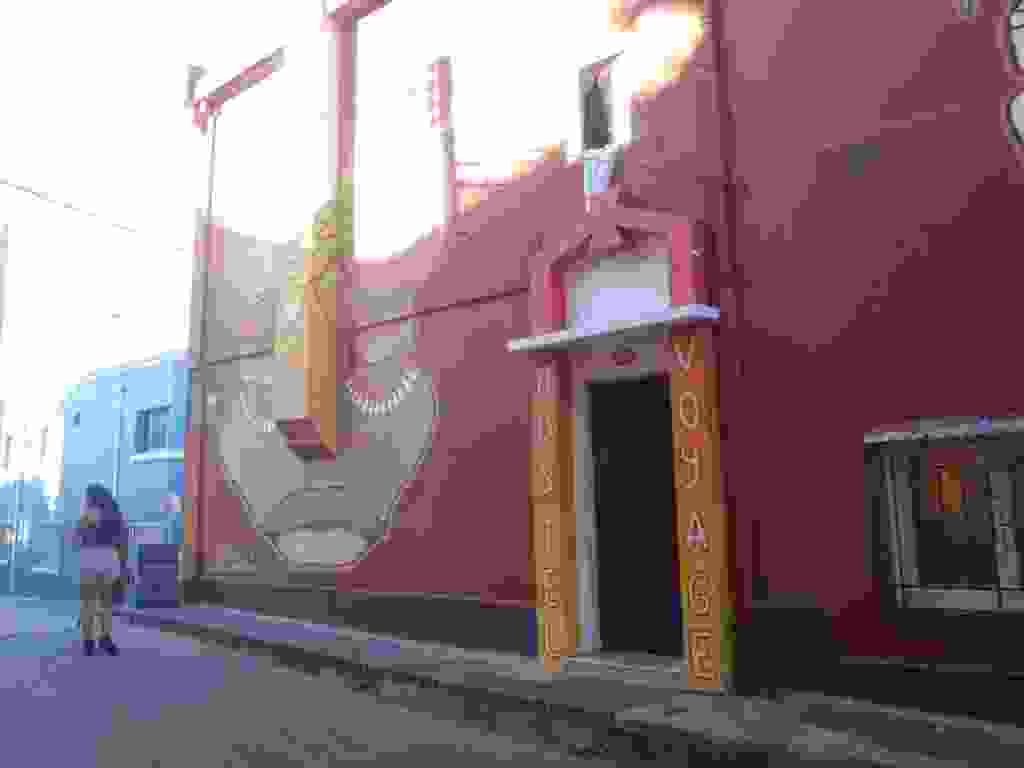
\includegraphics[width=\mywidth]{../wp-content/uploads/2015/03/P3092668-1024x768.jpg} \end{center}

 Un soir, un chilien a préparé un superbe plat de fruits de mer, poulet et pommes de terre. Le tout cuit au feu de bois, un régal !
\begin{center} 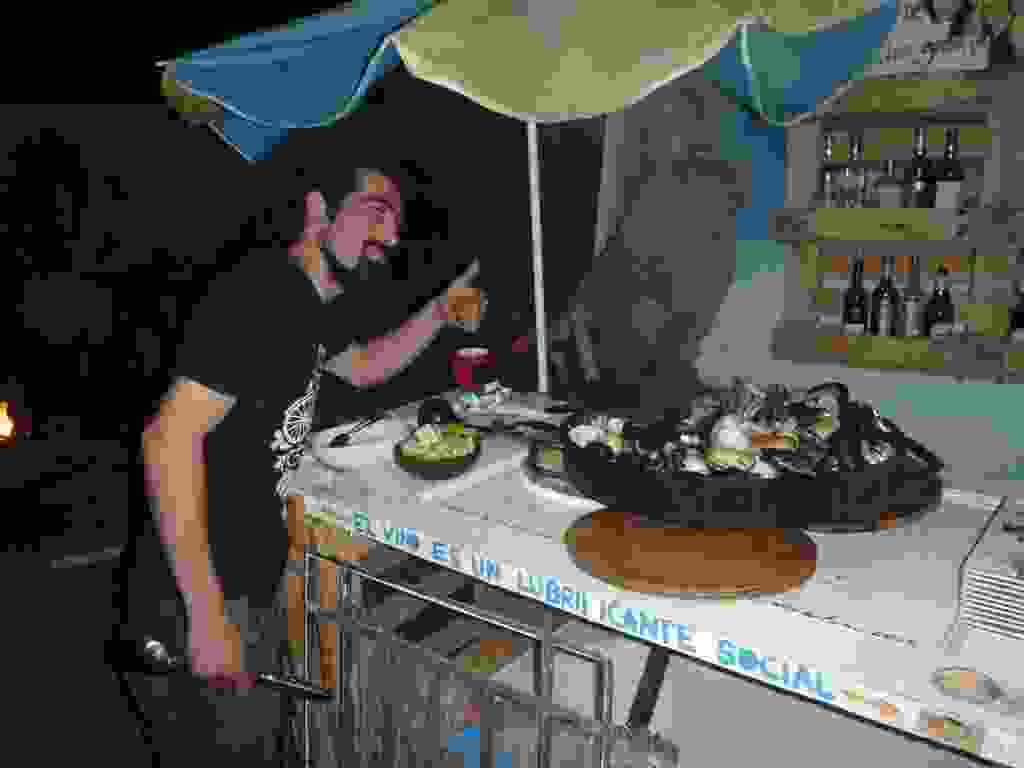
\includegraphics[width=\mywidth]{../wp-content/uploads/2015/03/P3112743-1024x768.jpg} \end{center}
\begin{center} 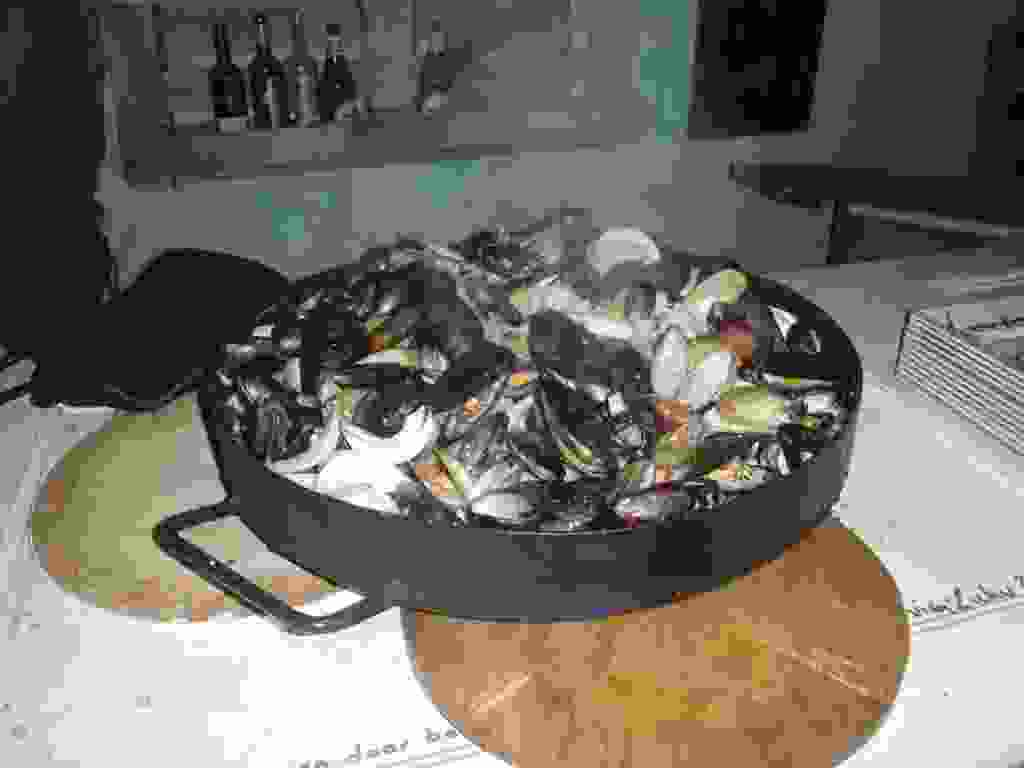
\includegraphics[width=\mywidth]{../wp-content/uploads/2015/03/P3112742-1024x768.jpg} \end{center}

 \subsection*{Viña del Mar}
 \`A peine à 10km de Valparaiso mais avec une ambiance totalement différente, ville balnéaire très propre avec de belles plages et des grands immeubles face à la mer.
\begin{center} 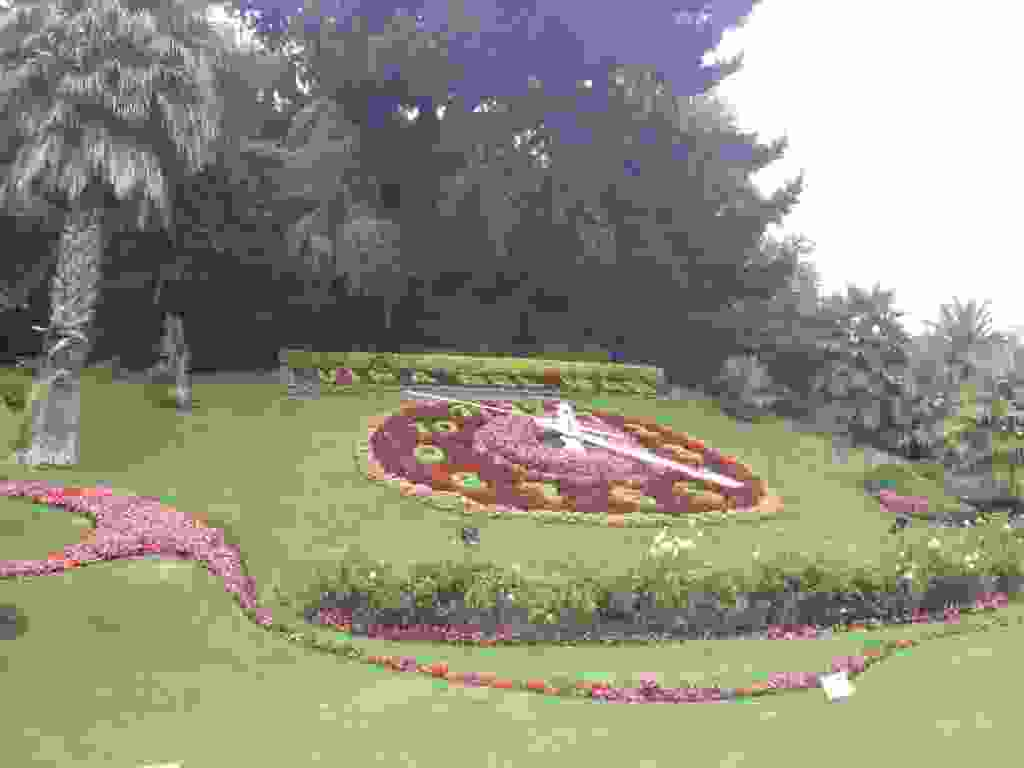
\includegraphics[width=\mywidth]{../wp-content/uploads/2015/03/P3102721-1024x768.jpg} \end{center}
\begin{center} 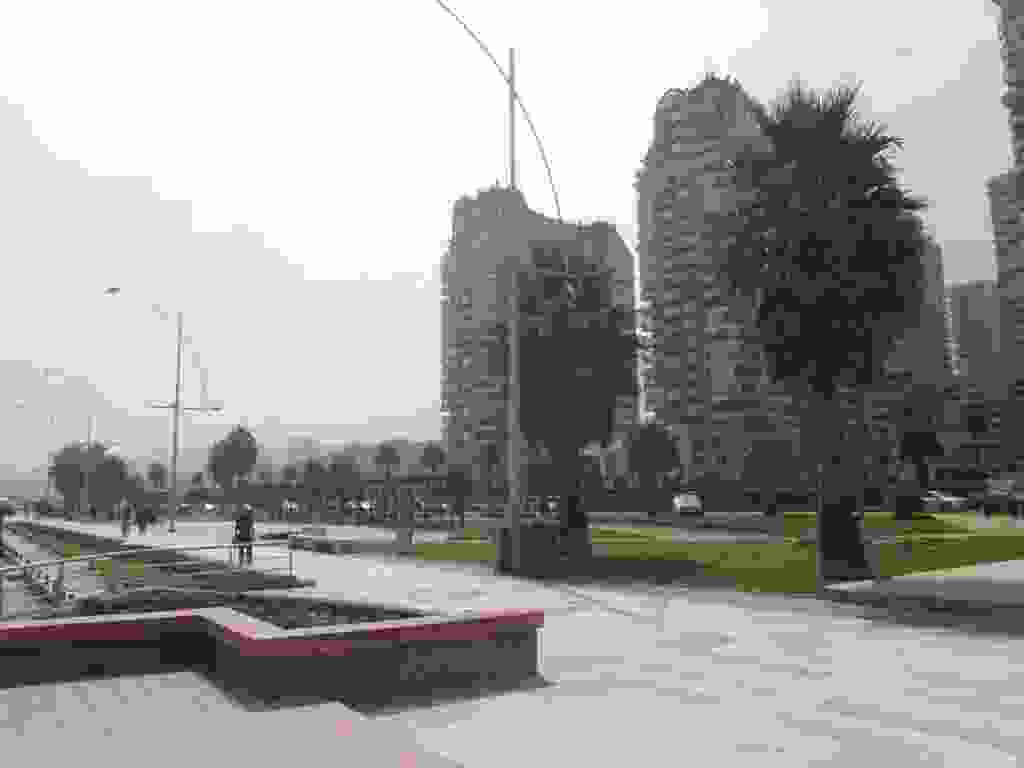
\includegraphics[width=\mywidth]{../wp-content/uploads/2015/03/P3102726-1024x768.jpg} \end{center}
\begin{center} 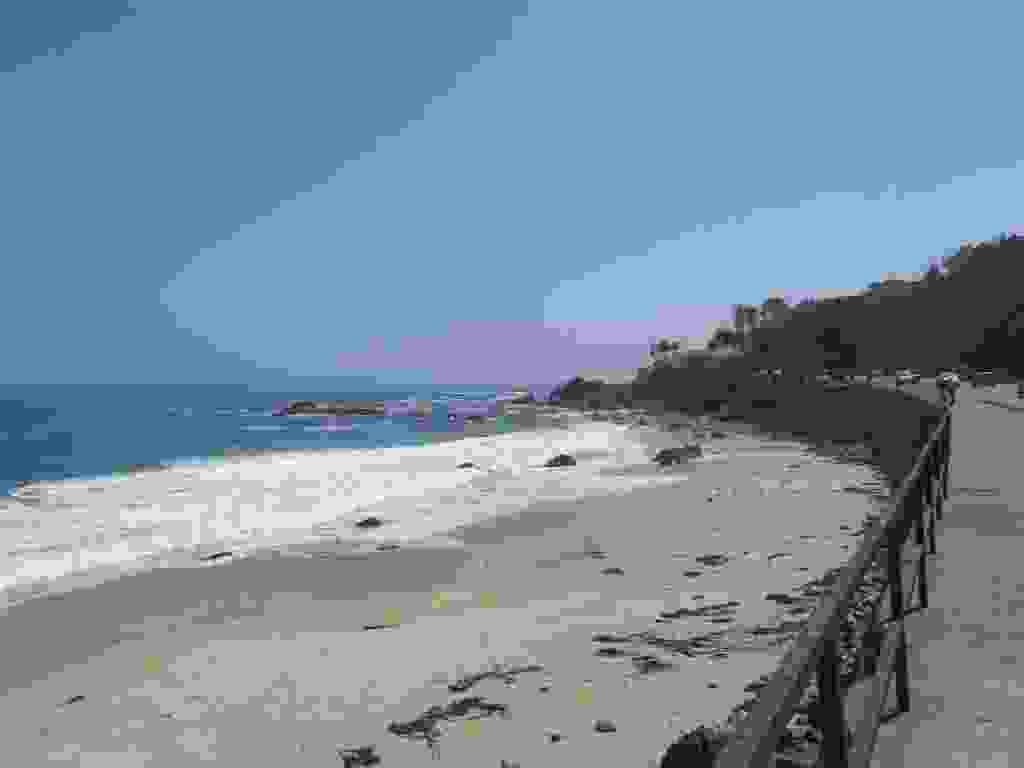
\includegraphics[width=\mywidth]{../wp-content/uploads/2015/03/P3102728-1024x768.jpg} \end{center}
\begin{center} 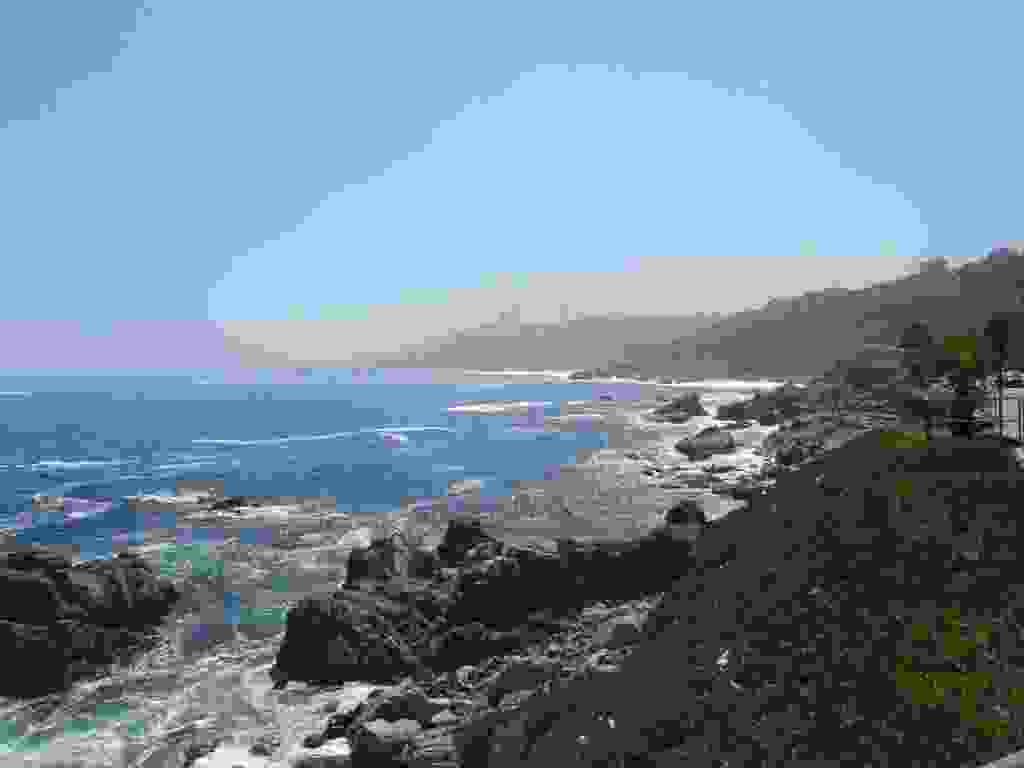
\includegraphics[width=\mywidth]{../wp-content/uploads/2015/03/P31027291-1024x768.jpg} \end{center}
\begin{center} 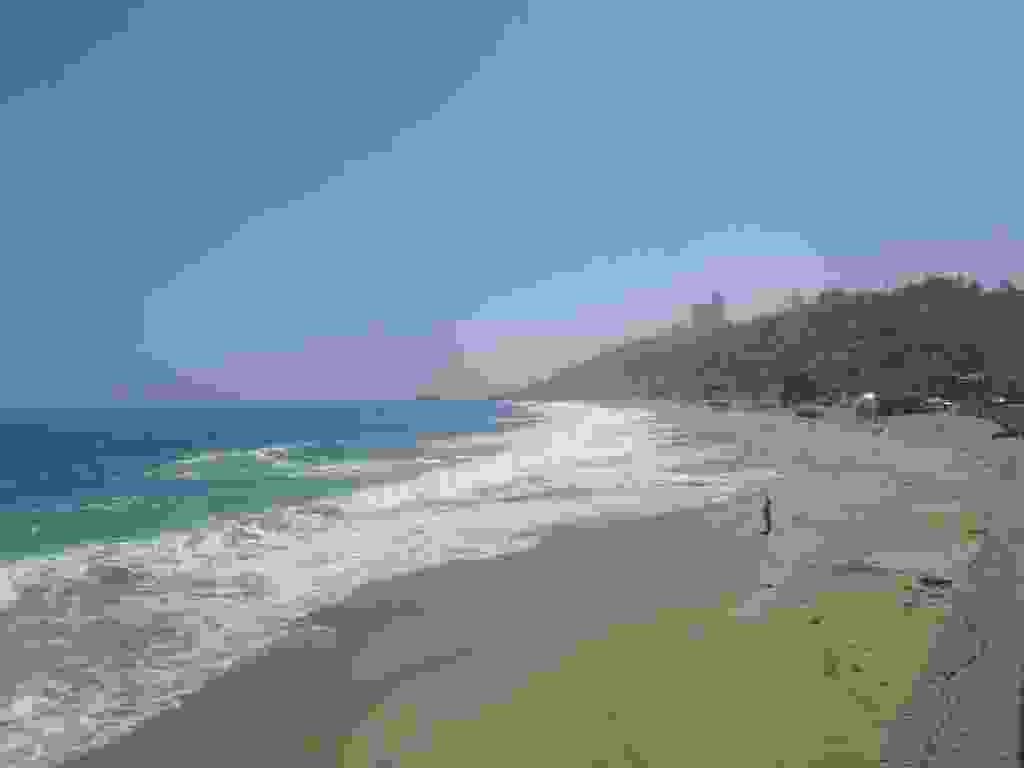
\includegraphics[width=\mywidth]{../wp-content/uploads/2015/03/P3102731-1024x768.jpg} \end{center}
\begin{center} 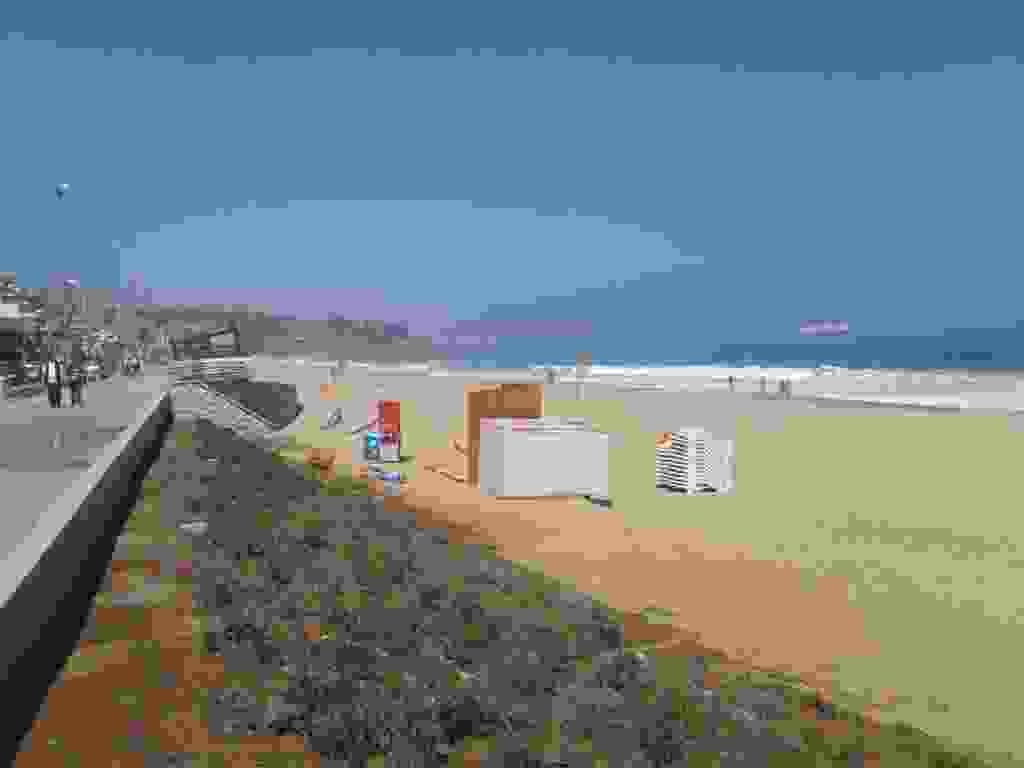
\includegraphics[width=\mywidth]{../wp-content/uploads/2015/03/P3102732-1024x768.jpg} \end{center}
\begin{center} 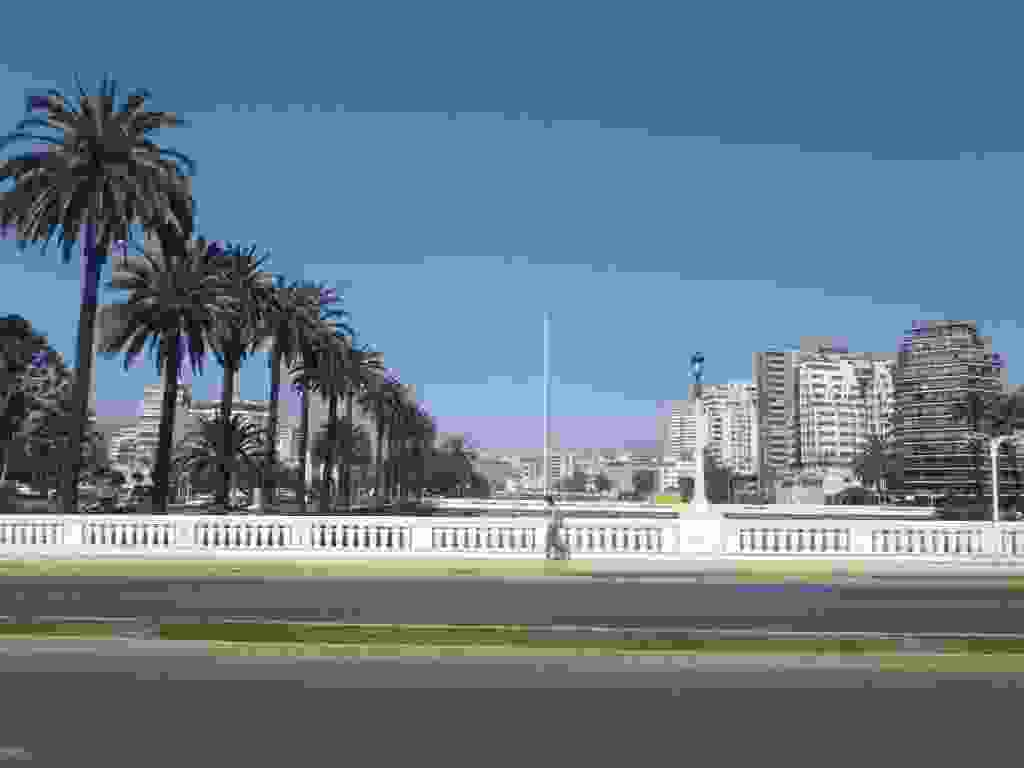
\includegraphics[width=\mywidth]{../wp-content/uploads/2015/03/P3102735-1024x768.jpg} \end{center}
\begin{center} 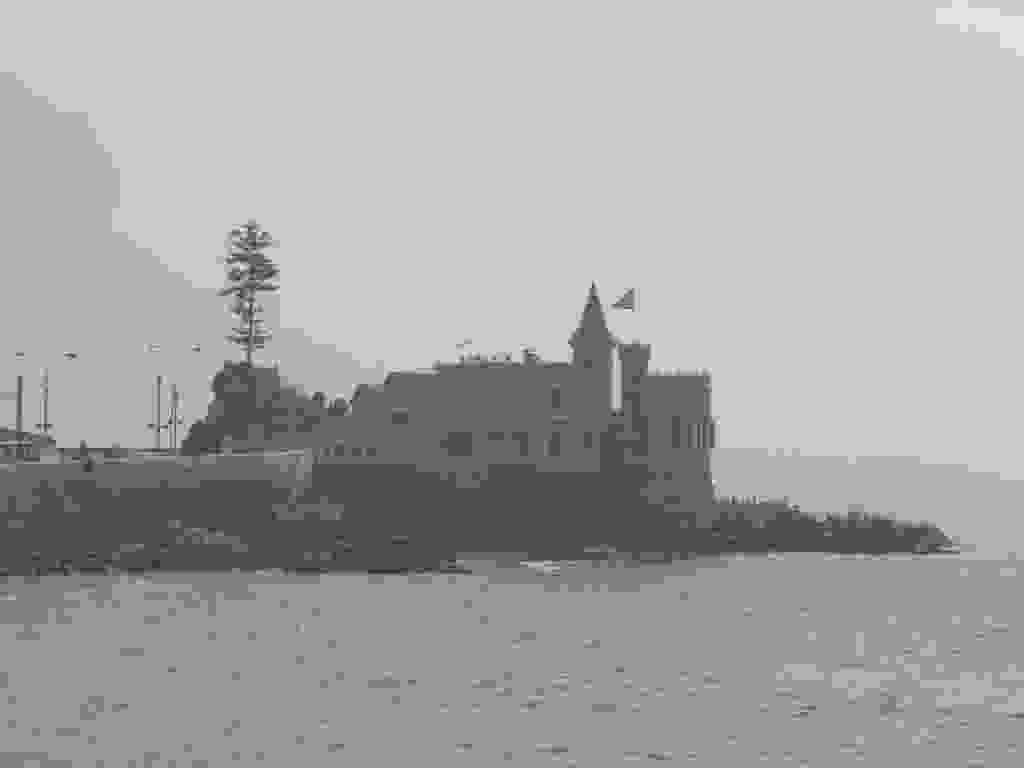
\includegraphics[width=\mywidth]{../wp-content/uploads/2015/03/P3102738-1024x768.jpg} \end{center}
\begin{center} 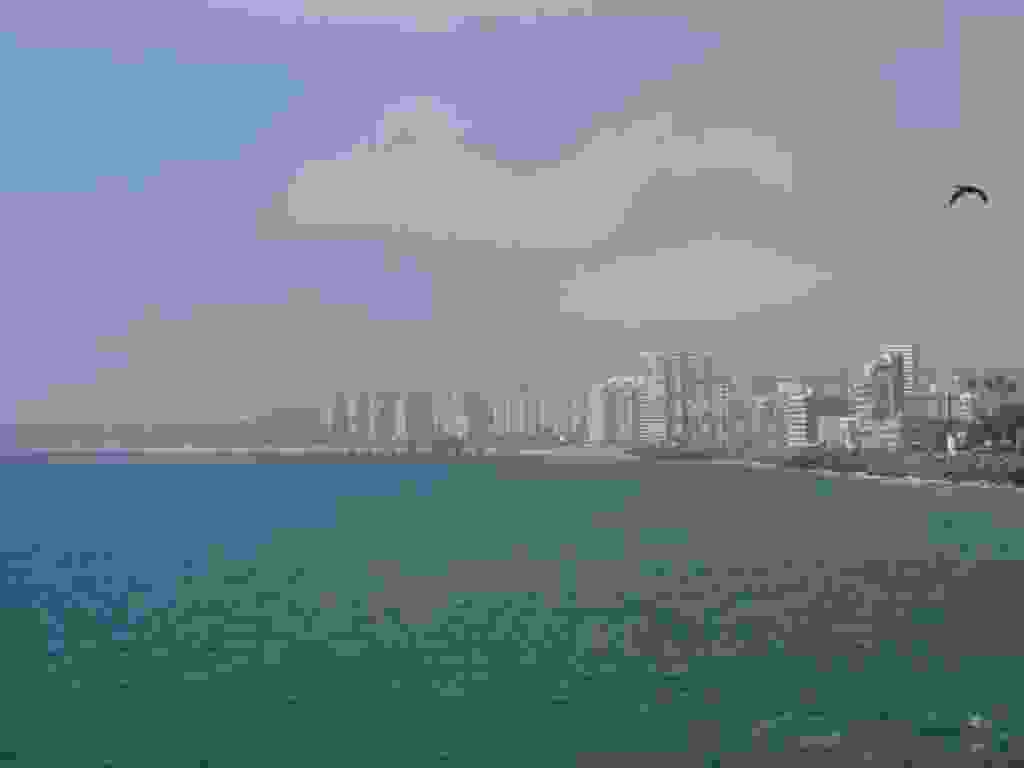
\includegraphics[width=\mywidth]{../wp-content/uploads/2015/03/P3102739-1024x768.jpg} \end{center}
\begin{center} 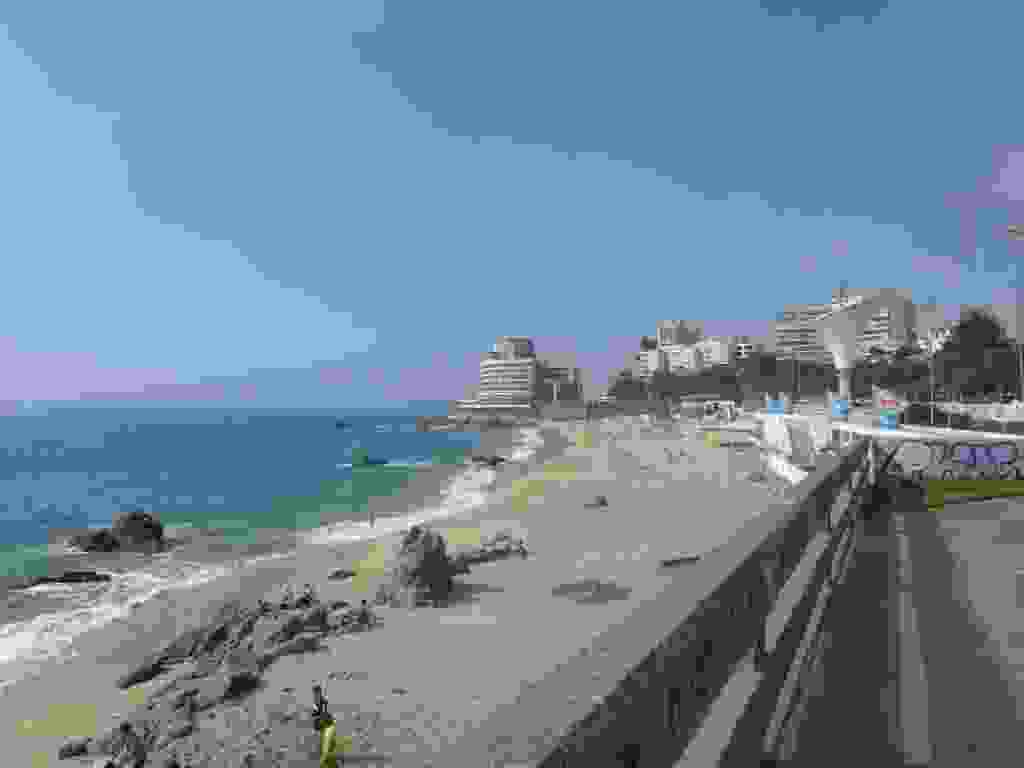
\includegraphics[width=\mywidth]{../wp-content/uploads/2015/03/P3102741-1024x768.jpg} \end{center}
